\chapter{Timing Domains and Synchronization}
\label{chap:timing}
% Traceability: ADR-001 ADR-003 ADR-004 ADR-005

The controller uses several clocks and synchronization signals for different jobs. They should not be treated as one timing system.

Detector sequencing needs a common, deterministic clock. Acquisition start and stop events must be associated with the same clock cycle on every participating board. Management and safety must continue if that distributed timing is lost. Power converters use another synchronization mechanism to make switching noise predictable.

Figure~\ref{fig:timing-domains} separates these functions.

\begin{figure}[htbp]
  \centering
  % Preserve the standard diagram font size; this narrow figure needs no enlargement.
  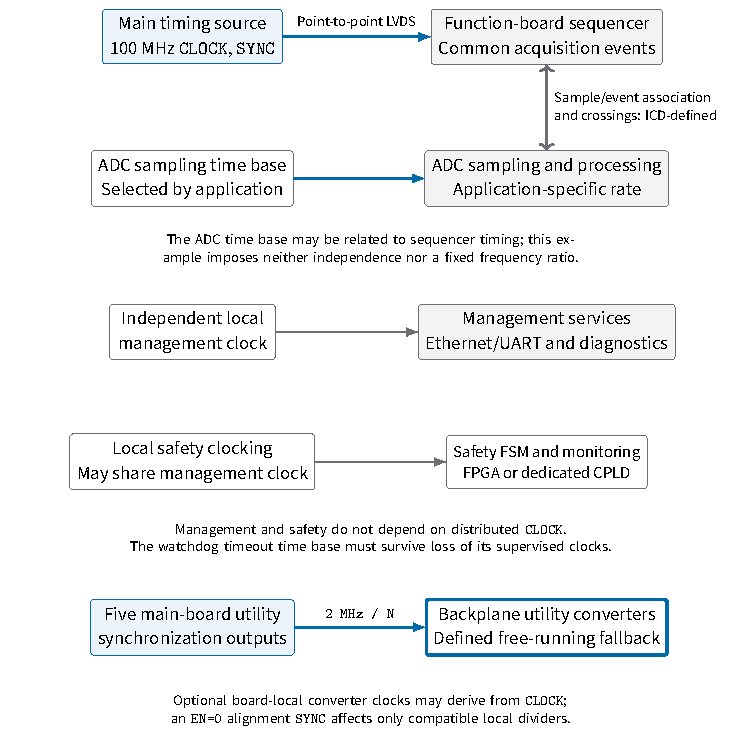
\includegraphics{figures/generated/timing_domains.tikz.pdf}
  \caption{Timing-domain relationships. The sequencer path is coherent across boards, local management remains independent, and utility-converter synchronization is a separate function.}
  \label{fig:timing-domains}
\end{figure}

\section{The Distributed Sequencer Clock}

The main board distributes a continuous 100~MHz \texttt{CLOCK} for detector sequencing. Function boards use the full-rate clock directly for timing-critical work. They may divide it by an integer for slower synchronous functions, but they do not recreate the 100~MHz clock by multiplying a slower reference.

Using the same full-rate source gives participating boards a common timing reference. A clock board can generate detector phases while a video board associates samples and processing windows with sequencer events. The exact local actions remain board-specific.

The architecture does not select the clock source, fanout device, receiver, or FPGA I/O method. Those choices must meet the instrument timing budget.

ADC sampling rate is application-specific; the 100~MHz sequencer clock does not impose a universal ADC rate. The video-board ICD defines the sampling time base and its relationship to acquisition events and processing windows, including any required clock-domain crossings. An ADC maximum supported rate is distinct from the selected operating rate.

\section{Point-to-Point Slot Distribution}

Each supported slot receives its own LVDS \texttt{CLOCK} pair and its own LVDS \texttt{SYNC} pair from the applicable fanout. The timing interface is point-to-point rather than a multidrop transmission line.

This avoids slot stubs and population-dependent loading. An empty slot does not change the electrical load seen by a populated slot. It also lets the timing design verify each source-to-receiver path with a clear endpoint.

Point-to-point does not mean that every path is automatically identical. Fanout delay, trace length, connectors, receivers, and environmental changes still contribute to the total timing budget. The ICD defines the electrical interface and the allowed path differences.

When a bridge extends timing to another backplane, the extension must still present point-to-point timing to each supported slot. The instrument design verifies all added propagation, skew, and clock-quality effects. The architecture does not require one universal multi-backplane topology.

\section{Acquisition SYNC and Cycle Agreement}

The \texttt{SYNC} signal carries acquisition start and stop events. A rising event starts acquisition behavior, and a falling event stops it. These events are timing-critical only where they enter the sequencer domain.

Main changes \texttt{SYNC} on a falling edge of the distributed 100~MHz \texttt{CLOCK}. Participating function boards capture the received level on the following rising edge. This nominal half-cycle separation prevents a transition from arriving close to the active edge that captures it. Without this rule, small path differences could make one board associate an event with the previous cycle while another chooses the next cycle.

The 180-degree relationship is therefore about selecting the same intended cycle. It is not a general requirement to phase-align every clock in the controller. The timing ICD still verifies the actual setup and hold margin after all source, fanout, routing, connector, receiver, skew, and environmental effects.

Timing-critical ADC controls, such as conversion-start signals, remain in deterministic sequencer-domain paths. Their exact FPGA implementation and constraints belong to the video-board design.

\section{Independent Management Clocking}

Each active board uses local clocking so management and safety functions can continue when the distributed acquisition clock disappears. The board can then detect timing loss, assert its local trip, retain diagnostics, communicate with the host, and participate in recovery. Management serves host supervision, diagnostics, Ethernet, and UART independently of acquisition timing.

Management may also need to know that acquisition has started or stopped. It receives the \texttt{SYNC} level or acquisition-event information through a reliable clock-domain crossing. Unlike the sequencer, management does not need to observe the event on the exact acquisition-clock cycle, so its clock does not require phase alignment with the distributed clock.

For example, the sequencer acts on \texttt{SYNC} at the specified clock edge; management subsequently records that acquisition has started. The reporting delay does not change when the sequencer acted. This management copy serves status and diagnostics, not timing-critical acquisition control.

A board may align a local clock for implementation convenience, but safety, communication, fault reporting, and recovery must remain available without that alignment or the distributed clock. Operational timeouts use the appropriate local time base; oscillator accuracy and timer values belong to the applicable ICDs.

Safety functions may share the management clock or use a separate local safety clock, including one in a dedicated CPLD. The watchdog timeout time base must remain operational when the clocks it supervises stop. A common oscillator for all these functions is not required.

\section{Clock-Loss Detection and Watchdog Evidence}

Clock loss and frozen processing are separate failures. A clock monitor detects loss of acquisition timing, while an independent watchdog detects when the processor or control logic stops refreshing it. Either can assert \texttt{OK} LOW and make the system safe, without waiting for the other or for the host.

On a function board, the clock monitor observes the distributed 100~MHz \texttt{CLOCK}; on main, it observes the external clock source. It uses independent local management or safety clocking, so it can still detect the loss when the acquisition clock stops. A disconnected clock cable therefore produces a clock-loss trip.

The processor or control logic periodically refreshes the watchdog as part of its normal execution. These refreshes are also called \emph{petting}. If execution freezes and refreshes stop, the watchdog times out and asserts its hardware trip. Refreshes use local clocking. An automatic pulse generator that keeps refreshing the watchdog after the processor freezes would defeat this protection.

A board may optionally align refresh transitions with the acquisition clock to make their switching activity more predictable for noise control. If the external clock disappears, refresh timing uses the local clock. If it returns, alignment may resume. These changes must not cause a false timeout or allow refreshes to continue without processor/control-logic execution. The watchdog's own timeout time base remains independent throughout.

For example, a disconnected acquisition-clock cable causes a clock-loss trip. A frozen processor that stops refreshing its watchdog causes a watchdog trip. Each failure has its own detector and diagnostic record.

Watchdog protection applies while armed and disarmed, with startup qualification preventing arming before protection is ready. Host-supervision timeout remains a separate rule that trips only while armed.

The board records clock loss and watchdog timeout separately. After a trip, the host uses the clock-loss record to investigate acquisition timing and the watchdog record to investigate processing and its refresh path. If both are recorded, both conditions were detected; the records do not establish their order. If the board is unreachable, its local records are unavailable. The shared safe response does not wait for diagnosis.

\section{Timing Loss and Recovery}

Loss of required acquisition timing trips the controller and removes detector-facing permission as described in Chapter~\ref{chap:safety}. The board management domains continue to operate.

Restoring the 100~MHz clock does not resume acquisition. The system remains in the safe error state until the host requests recovery. Boards clear retained evidence only at the allowed recovery point, requalify live timing, return to \texttt{IDLE}, and wait for a new arm request.

This rule prevents a loose cable, unstable source, or intermittent receiver from restarting detector activity as soon as a waveform happens to return.

\section{Utility-Converter Synchronization Is Separate}

The backplane utility converters do not use the 100~MHz detector sequencer interface. Main provides five separate point-to-point LVDS outputs for utility-converter synchronization.

During acquisition, each enabled switching channel uses a frequency of \texttt{2 MHz / N}, where the positive integer \texttt{N} and channel mapping are defined by the backplane ICD. Converter phase behavior is also an ICD decision. Forced continuous, fixed-frequency operation keeps the switching pattern predictable.

If synchronization is absent, the utility converter remains enabled and free-runs in a defined fixed-frequency continuous mode. This fallback is different from loss of the required detector sequencer clock. It does not create an uncontrolled rail or require processor intervention.

The converter synchronization settings remain fixed during acquisition. Chapter~\ref{chap:power} explains the noise-control reason for this choice.

\section{Optional Board-Local Converter Synchronization}

A function board may synchronize one or more compatible local converters when coherent switching improves detector performance. Their continuous switching references may be derived from the distributed \texttt{CLOCK} and, when appropriate, use the same \texttt{2 MHz / N} convention.

Whenever the system enters \texttt{START}, main sends one converter-alignment \texttt{SYNC} pulse while \texttt{EN=0}. A compatible function board recognizes any such pulse whether its own state is \texttt{START}, \texttt{IDLE}, or \texttt{ERROR}. It may then reset or align its local converter divider. The pulse does not clear a fault or change the board's safety state.

A board that requires this alignment completes any required settling before declaring itself ready. With \texttt{EN=1}, \texttt{SYNC} has acquisition meaning only and does not reset local converter timing. Boards that do not use this feature ignore the alignment pulse.

This use is optional and local to the board. Divider, phase, settling, filtering, and free-running fallback belong to the board ICD and design.

Optional converter timing does not change the acquisition \texttt{SYNC} capture rule and does not create another shared system state.

\section{Timing Budgets Belong to the Application}

The architecture defines which relationships must be controlled, but it does not set universal jitter, skew, or delay numbers. The acceptable values depend on the detector, ADC, FPGA, board count, routing, and selected clock components.

The timing ICD verifies the complete path from the source through fanout, backplane routing, connectors, receivers, FPGA logic and I/O, data converters, and detector interface circuits. A multi-backplane instrument includes the bridge and extension path in the same analysis.

This approach keeps the important concept fixed: all participating boards must select the intended acquisition cycle. The numerical budget remains with the interface and implementation that can be measured and verified.

\medskip
\noindent\textit{Chapter sources:} ADR-004 defines sequencer timing, acquisition \texttt{SYNC}, independent management clocks, clock-loss evidence, and multi-backplane timing. ADR-001 defines watchdog and fault evidence. ADR-003 defines acquisition and recovery behavior, and ADR-005 defines utility-converter synchronization.
